\documentclass[12pt]{article}
\usepackage[a4paper, margin=1in]{geometry} 
\usepackage{graphicx} 
\usepackage{hyperref}
\usepackage{float}
\usepackage{multicol}
\usepackage{multirow}
\usepackage{amsmath}
\usepackage[ruled]{algorithm2e}
\usepackage{amssymb}
\usepackage[font=small, labelfont=bf]{caption}
\usepackage[table,xcdraw]{xcolor}

\title{Lecture Notes for \\ INF281 Basics of Bioinformatics Sequence Analysis}
\author{Takaya Saito}
\date{}

\begin{document}

\pagenumbering{arabic}
\setcounter{page}{79}

\makeatletter 
\renewcommand{\thefigure}{\arabic{section}.\arabic{figure}}
\renewcommand{\thetable}{\arabic{section}.\arabic{table}}
\makeatother

%
% PART V
%
\setcounter{part}{4}
\part{}

%
% Construction of scoring matrix
%
\setcounter{section}{10}
\setcounter{figure}{0}
\setcounter{table}{0}
\section{Construction of scoring matrix}
%\documentclass[12pt]{article}
%\usepackage[a4paper, margin=1in]{geometry} 
%\usepackage{graphicx} 
%\usepackage{hyperref}
%\usepackage{float}
%\usepackage{multicol}
%\usepackage{multirow}
%\usepackage{amsmath}
%\usepackage[font=small, labelfont=bf]{caption}
%
%\begin{document}

%
% Scoring schemes for protein sequence alignment
%
\subsection{Scoring schemes for protein sequence alignment}
Applying an appropriate scoring scheme is critical to create biologically accurate alignments and phylogenetic trees. 

%
% Different types of scoring schemes for proteins
%
\subsubsection*{Different types of scoring schemes for proteins}
\begin{itemize}
\item Use of identity
\item Use of the genetic code
\item Use of a classification of amino acids
\item Scoring matrix
\end{itemize}

%
% Use of identity
%
\subsubsection*{Use of identity}
The score is calculated by counting identical amino acids. It is equivalent with a simple scoring scheme with match: 1, mismatch: 0, and gap penalty: 0.

%
% Example of "use of identity"
%
\subsubsection*{Example of ``use of identity''}
Calculate the SP score by counting identical amino acids. 

\begin{verbatim}
   Seq1 F-NV
   Seq2 FPN-
   Seq3 FC-V
\end{verbatim}

$\begin{aligned}
S(\bar{s}^1, \bar{s}^2) &= 2 \\
S(\bar{s}^1, \bar{s}^3) &= 2 \\
S(\bar{s}^2, \bar{s}^3) &= 1
\end{aligned} $

\bigskip 

$\begin{aligned}
S(\mathcal{A}) &= S(\bar{s}^1, \bar{s}^2) + S(\bar{s}^1, \bar{s}^3) + S(\bar{s}^2, \bar{s}^3) = 2 + 2 + 1 = 5
\end{aligned} $

\bigskip 
Score: 5

%
% Use of the genetic code
%
\subsubsection*{Use of the genetic code}
The score is based on the distance between two amino acids at the codon level. 

%
% Example of "use of the genetic code"
%
\subsubsection*{Example of ``use of the genetic code''}

\begin{verbatim}
   Seq1 FFFF
   Seq2 FCNG
\end{verbatim}

\begin{verbatim}
   Phe (UUU, UUC) & Phe (UUU, UUC): 3
   Phe (UUU, UUC) & Cys (UGU, UGC): 2
   Phe (UUU, UUC) & Asn (AAU, AAC): 1
   Phe (UUU, UUC) & Glu (GAA, GAG): 0
\end{verbatim}

Score: 6

%
% Use of a classification of amino acids
%
\subsubsection*{Use of a classification of amino acids}
The score is based on the physio-chemical properties. For example, AACH (amino acid class hierarchy) can be used as a scoring scheme.
\bigskip 

\begin{figure}[H]
  \centering
      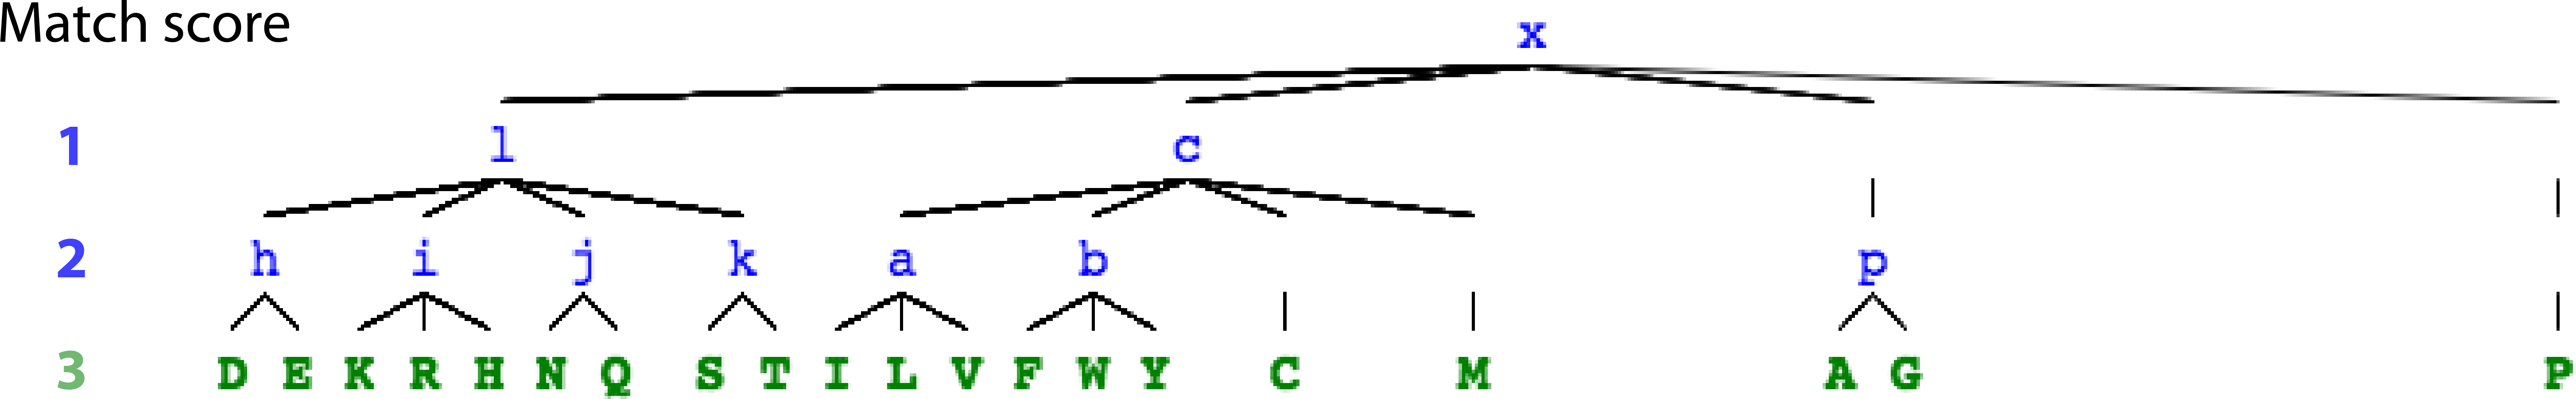
\includegraphics[width=0.75 \textwidth]{fig11/aach.png}
  \caption{Example of amino acid class hierarchy (AACH)}
\end{figure}

%
% Example of " Use of a classification of amino acids"
%
\subsubsection*{Example of ``Use of a classification of amino acids''}
Calculate the score by using AACH. 

\begin{verbatim}
   Seq1 DDDP
   Seq2 DEKD
\end{verbatim}

D \& D: 3, D \& E: 2, D \& K: 1, P \& D: 0

Score: 6

%
% Scoring matrix
%
\subsubsection*{Scoring matrix}
\begin{itemize}
\item DNA/RNA: 4 $\times$ 4
\item Protein: 20 $\times$ 20
\end{itemize}

%
% PAM and BLOSUM 
%
\subsubsection*{PAM and BLOSUM}

BLAST parameters

\begin{figure}[H]
  \centering
      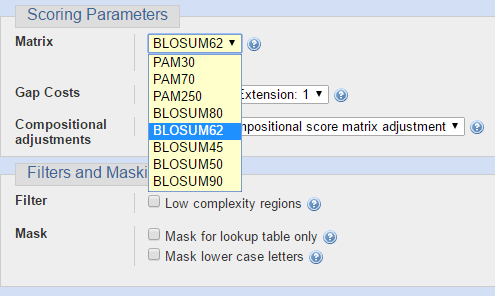
\includegraphics[width=0.6 \textwidth]{fig11/blast_pam_blosum.png}
  \caption{BLAST score parameters (source: \href{http://blast.ncbi.nlm.nih.gov})}
\end{figure}

\noindent
Correspondence between PAM and BLOSUM

\begin{table}[H]
\centering
\begin{tabular}{lll}
PAM 120    & PAM 160    & PAM 250    \\
BLOSUM 80 & BLOSUM 62 & BLOSUM 45
\end{tabular}
\end{table}

%
% Types of substitutions 
%
\subsubsection*{Types of substitutions}
There are several types of substitutions between two sequences from the common ancestor. 
\begin{figure}[H]
  \centering
      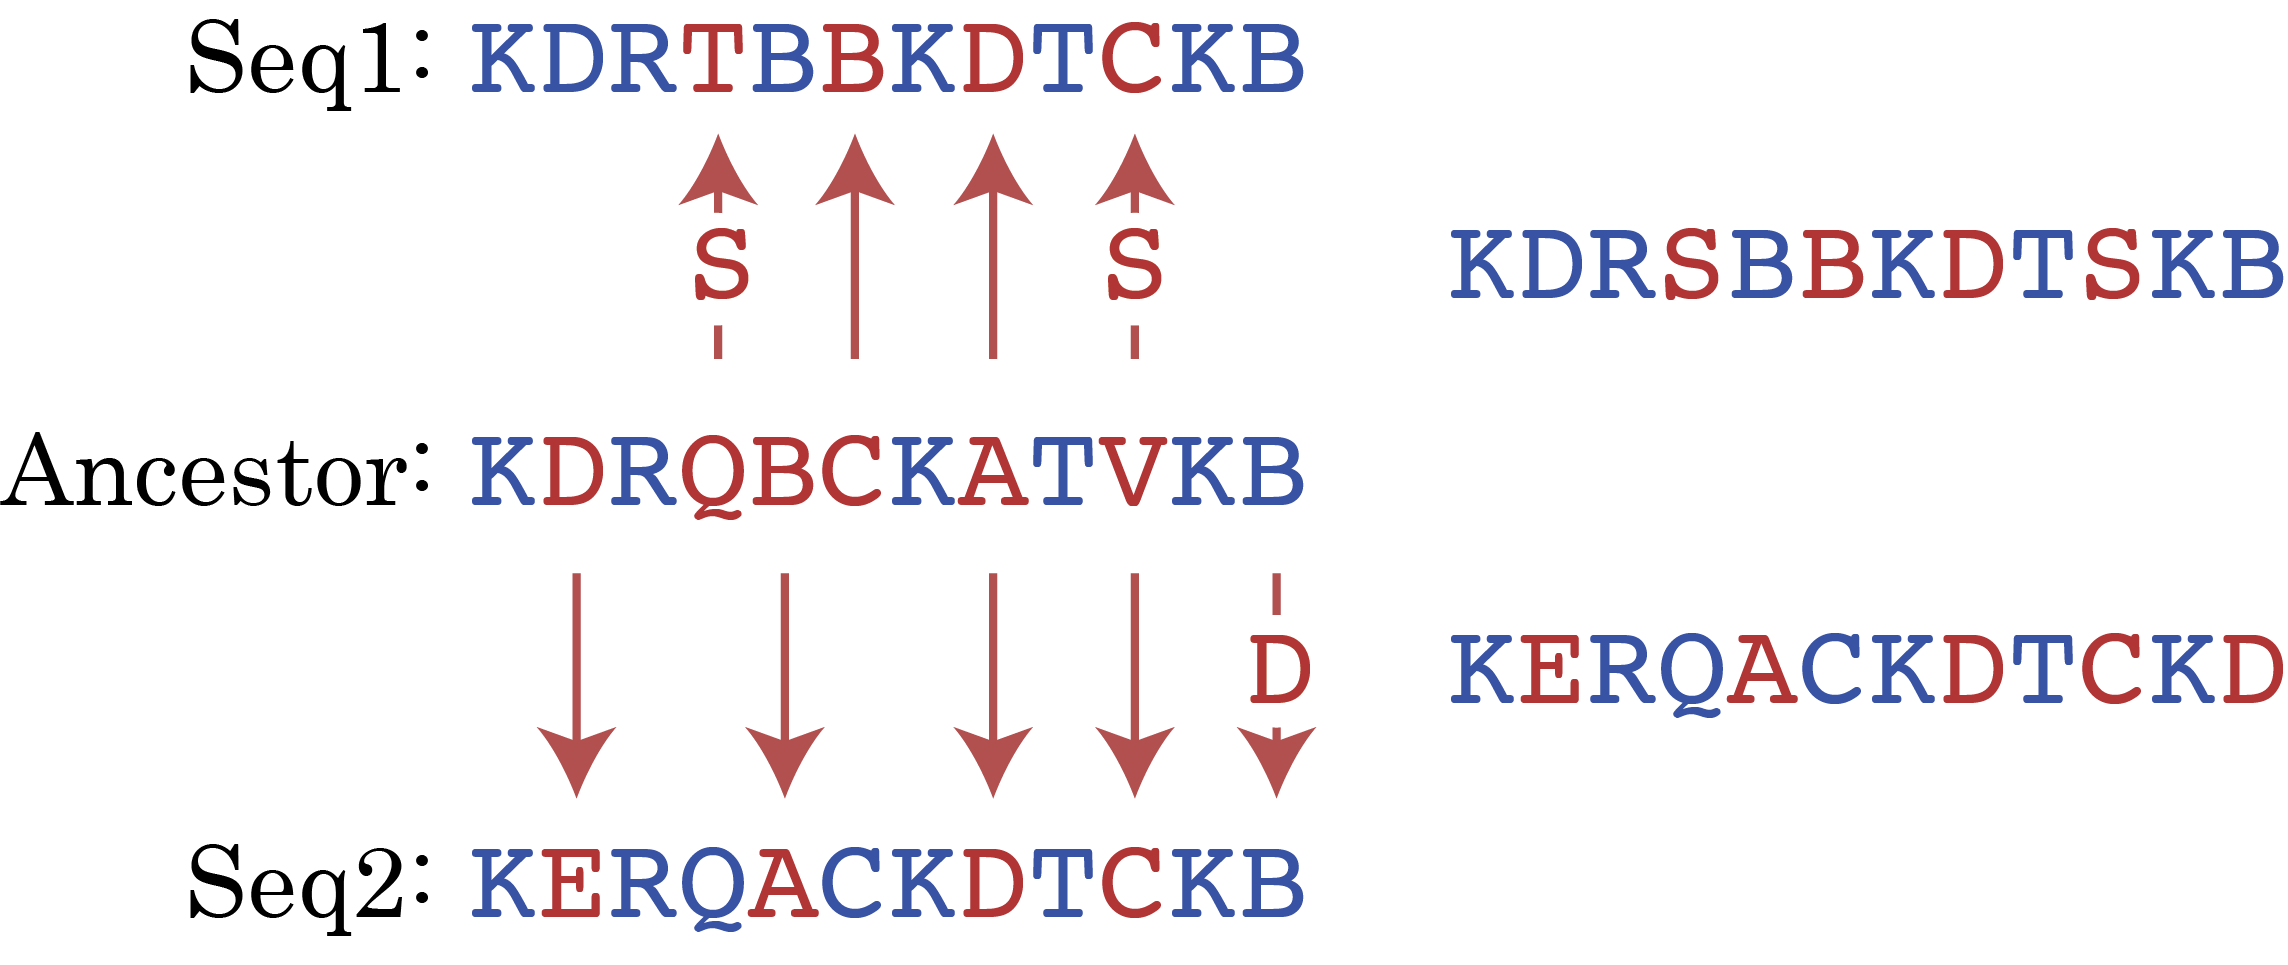
\includegraphics[width=0.6 \textwidth]{fig11/potential_mutations.png}
  \caption{Different types of substitutions}
\end{figure}

%
% Exercise \thesection.1
%
\subsubsection*{Exercise \thesection.1}
Calculate the score of the alignment by using different scoring schemes.

\begin{verbatim}
   Seq1 K-RI
   Seq2 KDCC
\end{verbatim}

\begin{itemize}
\item Use the identity.
\bigskip 

\item Use the genetic code.

\begin{table}[H]
\centering
\begin{tabular}{|l|l|l|}
\hline
K & Lys & AAA, AAG      \\ \hline
D & Asp & GAU, GAC      \\ \hline
R & Arg & CGU, CGC, CGA \\ \hline
I & Ile & AUU, AUC AUA  \\ \hline
C & Cys & UGU, UGC      \\ \hline
\end{tabular}
\end{table}

\item Use AACH.
\bigskip 

\end{itemize}

\bigskip 

%\end{document}

%\documentclass[12pt]{article}
%\usepackage[a4paper, margin=1in]{geometry} 
%\usepackage{graphicx} 
%\usepackage{hyperref}
%\usepackage{float}
%\usepackage{multicol}
%\usepackage{multirow}
%\usepackage{amsmath}
%\usepackage[font=small, labelfont=bf]{caption}
%
%\begin{document}

%
% PAM – accepted mutations
%
\subsection{PAM – accepted mutations}
PAM is a popular scoring scheme for protein sequence alignments. It is based on substitution matrices created from experiment data.

%
% Accepted point mutations
%
\subsubsection*{Accepted point mutations}
\begin{itemize}
\item Independent of positions and neighbor residues
\item Independent from previous mutations at the same position
\item Biological clock is assumed (the rate of mutations is constant)
\end{itemize}

%
% PAM (point accepted mutation) 
%
\subsubsection*{PAM (point accepted mutation)}
One PAM means one accepted point mutation per 100 residues. 

\noindent
Resources of constructing a PAM score
\begin{itemize}
\item 34 super-families
\item 71 groups of homologous sequences (85\% identity) 
\end{itemize}

%
% Preparations for constructing a PAM score
%
\subsubsection*{Preparations for constructing a PAM score}
Counting the number of mutations is the fist step to make a PAM score. Several sub-steps are involved.

\begin{itemize}
\item Create a phylogenetic tree
\item Estimate ancestor sequences
\item Count all occurrences of mutations
\end{itemize}

%
% Frequencies of estimated mutations
%
\subsubsection*{Frequencies of estimated mutations}
Frequencies of estimated mutations are counted in internal nodes of the reconstructed tree. \\

$\begin{aligned}
f_{ab} &: \text{The number of mutations from } a \text{ to } b \text{ or from } b \text{ to } a \\
f_{a} &: \text{The total number of mutations in which a takes part} \\
f & : \text{Twice the total number of mutations}
\end{aligned} $

%
% Example of frequency calculation
%
\subsubsection*{Example of frequency calculation}
Calculate $f_{CA}$, $f_{C}$, and $f$ from the phylogenetic tree and the table below.

\begin{figure}[H]
  \centering
      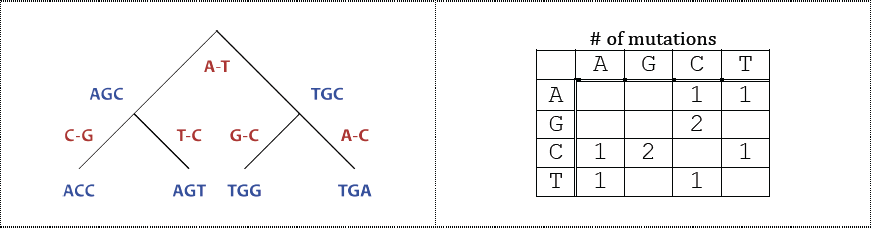
\includegraphics[width=0.75 \textwidth]{fig11/scoring_mat_frequency_example.png}
  \caption{Phylogenetic tree and a table of the number of mutations}
\end{figure}

$\begin{aligned}
f_{CA} &=1 \\
f_{C} &= 1 + 2 + 1 = 4\\
f &= 10
\end{aligned} $

%
% Background frequencies
%
\subsubsection*{Background frequencies}
The background probabilities are calculated from the data source. 

$\begin{aligned}
p_a &: \text{The relative occurrence of a in the observed sequences} 
\end{aligned} $

%
% Example of background frequencies
%
\subsubsection*{Example of background frequencies}
Calculate $p_G$ from the sequences below.

\begin{verbatim}
   Seq1 ACC
   Seq2 AGT
   Seq3 TGG
   Seq4 TGA
\end{verbatim}

$p_G = \dfrac{4}{12} \approx 0.333$

\bigskip 

%\end{document}


\end{document}
